\documentclass[border=4pt]{standalone}
\usepackage{tikz}
\usetikzlibrary{arrows.meta}
\definecolor{orangeText}{HTML}{E3A063}
\definecolor{orangeDim}{HTML}{A87A4E}
\begin{document}
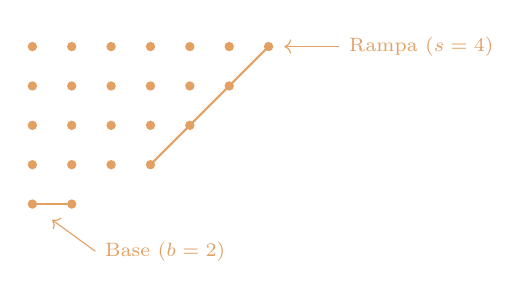
\begin{tikzpicture}[color=orangeText, scale=0.5,dot/.style={circle,fill,inner sep=1.2pt}]
  % partition 7+6+5+4+2 -> rows lengths, top row first
  \foreach \len [count=\r from 0] in {7,6,5,4,2} {
    \foreach \c in {1,...,\len} \node[dot] at (\c,-\r) {};
  }
  % ramp: from last point of first row (7,0) diagonal down-left: (7,0),(6,-1),(5,-2),(4,-3)
  \draw[thick] (7,0) -- (4,-3);
  \draw[thick] (1,-4) -- (2,-4);
  \draw[<-] (7.4,0) -- (8.8,0) node[right] {\scriptsize Rampa ($s=4$)};
  \draw[<-] (1.5,-4.4) -- (2.6,-5.2) node[right] {\scriptsize Base ($b=2$)};
\end{tikzpicture}
\end{document}
